\begin{figure}[t]
    \centering
    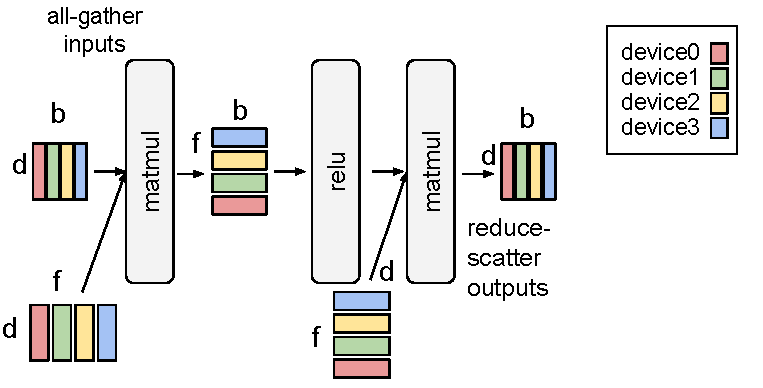
\includegraphics[width=0.6\textwidth]{figures/shard3b.pdf}
    \caption{4-way in-layer model parallelism with fully partitioned activations used to scale the 3B model training. The figure shows a simplified Transformer feed-forward layer (with the sequence dimension omitted); each color represents data on one device. We also use 128-way data parallelism.}
    \label{figs:shard3b}
\end{figure}

\section{Scaling}
We implement our models in Lingvo~\cite{shen2019lingvo} and scale with GSPMD~\cite{xu2021gspmd} on CloudTPUv4 hardware for both training and inference. GSPMD is an XLA compiler-based model partitioning system that allows us to treat a cluster of TPUs as a single virtual device and use \emph{sharding annotations} on a few tensors to instruct the compiler to automatically distribute data and compute on thousands of devices.

\textbf{Training.}
We train both 350M and 750M models simply with data parallelism. For the 3B model, we use 4-way in-layer model parallelism (see Figure~\ref{figs:shard3b}), and 128-way data parallelism. Partitioning a single dimension in each tensor is sufficient to scale a 3B model. The model weights are partitioned on the feed-forward hidden dimension and the number of attention heads dimension; the internal activation tensors of the feed-forward and attention layers are also partitioned on the hidden and heads dimensions. One difference from Megatron-LM~\cite{megatron} is we fully partition the output activations of feed-forward and attention layers on a different dimension, with the details illustrated as the \emph{finalized 2d sharding} in the GSPMD work~\cite{xu2021gspmd}. This strategy will result in \texttt{ReduceScatter} and \texttt{AllGather} communication patterns instead of \texttt{AllReduce}, which significantly reduce peak activation memory.

\begin{figure}[t]
    \centering
    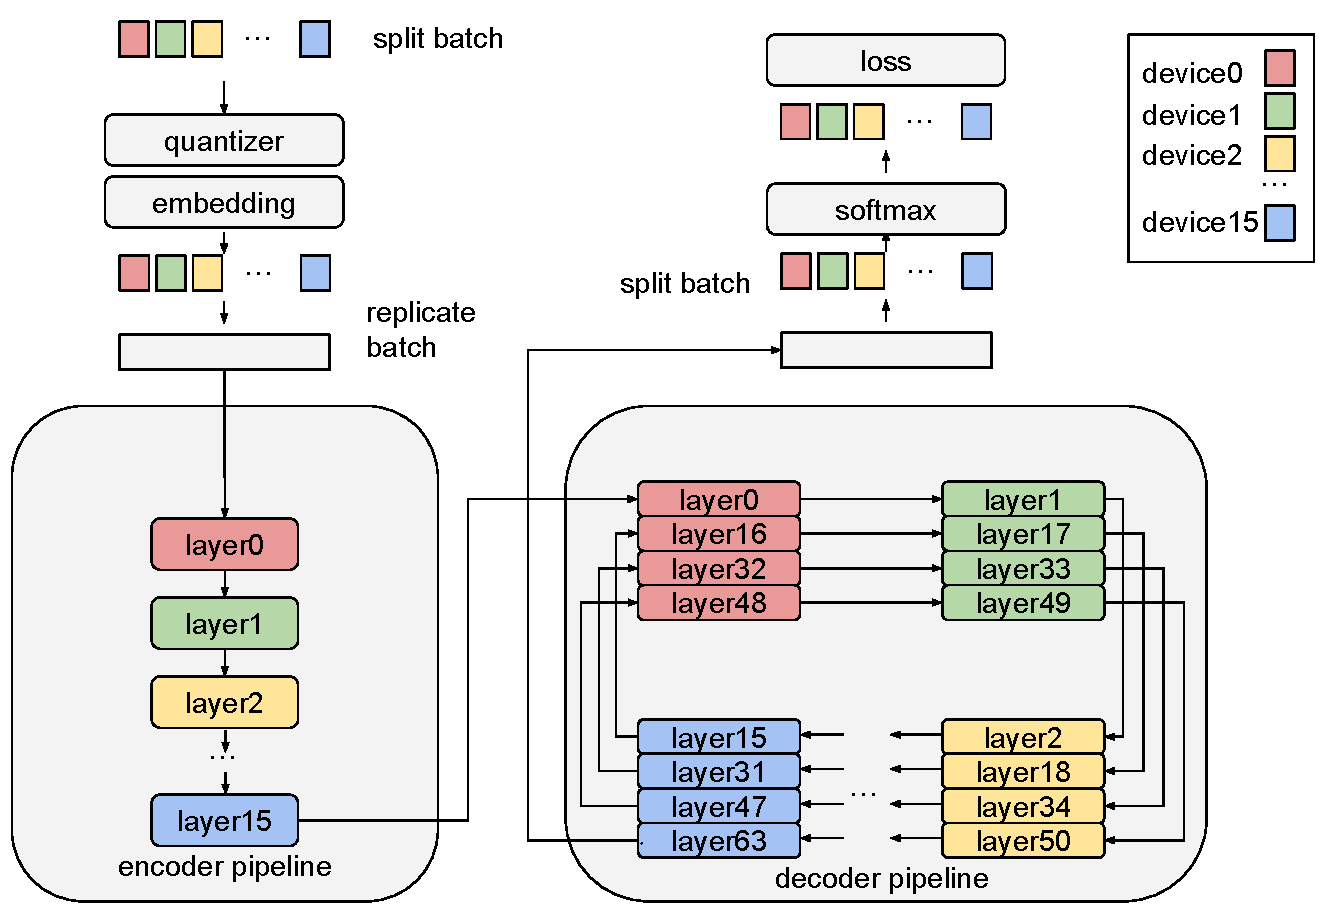
\includegraphics[width=0.8\textwidth]{figures/pipeline.pdf}
    \caption{An illustration of 16-stage GSPMD pipelines used to scale the 20B model training. The figure shows how the 16 devices are used for data parallelism in the quantizer, embedding and softmax layers, but repurposed for pipelining in the encoder and decoder layers. Each color represents data or layer assigned to one device. The decoder uses 4-round circular schedule to further reduce the pipeline bubble ratio. On top of this, we use additional 64-way data parallelism for all layers.}
    \label{figs:pipeline}
\end{figure}


The 20B model has 16 encoder layers, and 64 decoder layers (see Table~\ref{tabs:bdraw_variants}). The size of the weights per layer is moderate (as opposed to being very wide), which makes pipeline parallelism~\cite{gpipe} a good option for scaling. We use a generic pipelining wrapper layer allowing us to specify a single-stage program, which will later be automatically transformed into a multi-stage pipelining program; the wrapper layer uses vectorization and shifting buffers to reduce pipelining into a tensor partitioning problem (see Section 3.3 of~\cite{xu2021gspmd}). Thus, all lower-level infrastructure can be reused for pipelining. There are two additional benefits in adopting GSPMD pipelining: 1) it allows us to conveniently configure pipelines within model sub-components, simplifying the overall complexity for encoder-decoder models, and 2) since pipelining is implemented as tensor partitioning on vectorized programs, we can reuse the same set of devices for other types of parallelism outside the transformer layers.

We configure the model to have separate encoder and decoder pipelines, each with 16 stages. We also use 64-way data parallelism in addition to pipelining. However this makes per-core batch size small, exposing an additional challenge of excessive pipeline stalls due to inter-stage data dependency (known as \textit{bubbles} in pipeline parallelism~\cite{gpipe}). To reduce the ratio of bubbles, we adapt the \emph{circular schedule} as described in \cite{xu2021gspmd} in the decoder pipeline (a similar technique was also proposed in \cite{megatron21}), where the 4 layers in each stage are executed in a round-robin order. Outside the encoder and decoder, we use the same set of devices to do data parallelism instead of pipelining for the embedding, softmax, and image tokenizer layers. Figure~\ref{figs:pipeline} illustrates the overall distributed training strategy.

During training, Adafactor~\cite{shazeer2018adafactor} optimizer is used to save memory with $\beta_1 = 0.9$, $\beta_2 = 0.96$ and decoupled weight decay value of $4.5\times 10^{-2}$. The first moments of optimizer slot variables are also quantized from float32 to int8. We use default dropout ratio 0.1 for all models in both encoder and decoder. A deterministic version of dropout layer as well as a vectorized version of Adafactor optimizer are used in the 20B model to enable training pipelined models. Data types are cast to bfloat16 for attention projection and feed-forward transformers layers, while all layer norms and model output are kept as float32. We use a default learning rate of 4.5e-5 and exponential learning rate schedule with 5,000 warm-up steps. Exponential decaying starts at training steps 85,000 with a total of 450,000 steps and final ratio of 0.025. We use a global batch size of 8192 during training. We do not use exponential moving average of the model weights to save device memory. Conv-shaped sparse attention is used in the decoder transformers, similar to DALL-E~\cite{ramesh2021zero} (Appendix B.1. Architecture, Fig. 11). We additionally clip gradient norm to a value of 4.0 to stabilize the training, especially at the beginning. At the output of both the encoder and decoder, we apply an additional layer normalization.

\textbf{Inference.} Our primary goal for inference optimization is to speed up small-batch image generation. We choose in-layer model parallelism for both the 3B and 20B models. As opposed to training, we do not fully partition the output activations for feed-forward and attention layers for inference; this is because 1) each step of the autoregressive decoding produces much smaller tensors and (at the time of writing) \texttt{AllReduce} performs better on small data, 2) activation memory is not a concern during inference, which does not have a backward pass.